\section{Model matematyczny}
\label{sec:model}

W pierwszej kolejności postanowiono wyznaczyć model matematyczny obiektu sterowania. Dla tego modelu wyznaczane będzie optymalne sterowanie. Podstawową pracą z której korzystano do tego zadania jest \cite{Babazadeh}. Założono, że napęd stanowią silniki prądu stałego. Model takiego silnika w postaci równań stanu można przedstawić w następujący sposób:
\begin{equation}
\dot{x}=
\begin{bmatrix}
	\frac{R}{L} & \frac{k_e}{L} \\
	\frac{k_m}{I_r} & -\frac{k_e}{I_r}
\end{bmatrix}
x+
\begin{bmatrix}
	\frac{1}{L} & 0 \\
	0 & -\frac{1}{I_r}
\end{bmatrix}
u
\label{eq:dc_model_x}
\end{equation}
\begin{equation}
y=
\begin{bmatrix}
	0 & 1
\end{bmatrix}
x
\label{eq:dc_model_y}
\end{equation}
\noindent Gdzie:\newline
\(x=
\begin{bmatrix}
	i \\
	\omega
\end{bmatrix}\) jest wektorem zmiennych stanów.\newline
\(i\) jest prądem silnika.\newline
\(\omega\) jest prędkością obrotową.\newline
\(u=
\begin{bmatrix}
	V \\
	\tau
\end{bmatrix}\) jest wektorem wejść modelu.\newline
\(V\) jest napięciem podawanym na silnik.\newline
\(\tau\) jest momentem obciążenia mechanicznego.\newline
\(I_r\) jest momentem bezwładności przeniesionym na wał silnika.\newline
\(L\) jest induktancją.\newline
\(R\) jest rezystancją.\newline
\(k_e\) jest stałą elektromotoryczną.\newline
\(k_r\) jest stałą momentu silnika.

\paragraph*{}
Na rysunku \ref{fig:model_kola} przedstawiono rozkłady sił działających na koła omawianego pojazdu.

\begin{figure}[h]
	\centering
	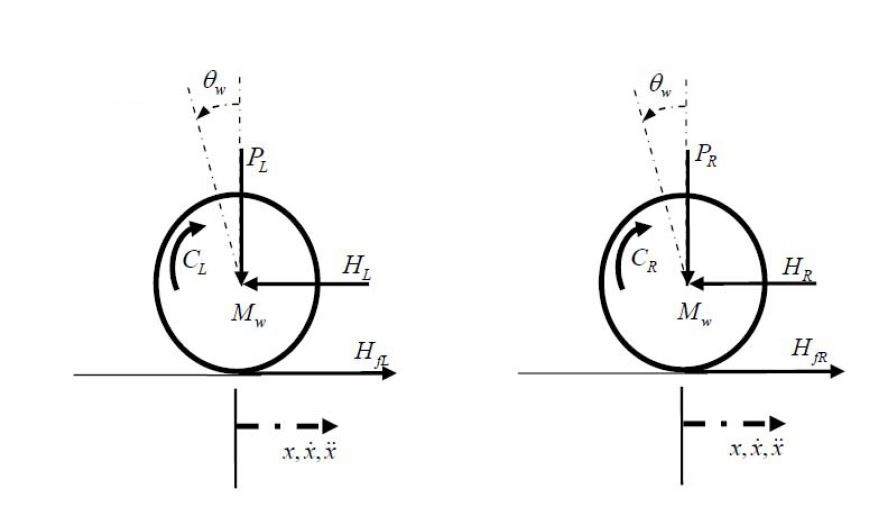
\includegraphics[width=4in]{Figures/model_kola.jpg}
	\captionsource{Siły działające na lewe i prawe koło pojazdu.}{\cite{Babazadeh}}
	\label{fig:model_kola}
\end{figure}